\chapter{System Architecture}
\label{sec:sysarchitecture}

To design a system fulfilling the requirements listed in \ref{sec:requirements}, we start from the bottom by first choosing its basic building blocks, and then we explore the different ways in which they can be assembled.
Finally we show an overview of the final system.
By the requirements, we only consider open-source technologies.


\section{Choice of Open-Source Technologies}

% outline
The choice of the open-source technologies to use depends mainly on the clinical research platforms that we aim to support.
First we review those platforms, then we explore existing open-source front end systems in hope of determining if one of them fits the requirements of our solution.
Finally we motivate the delegation of identity and access management to an identity provider, and choose a software that implements it.

\subsection{Clinical Research Platforms: i2b2, tranSMART and MedCo}

% what is a clinical research platform
A clinical research platform is a back end software (i.e. running on a server and serving requests to clients), that stores any kind of medical data and can answer queries, with the purpose of identifying patient cohorts, and possibly performing analysis on those data.

% use-case 
Queries on this data can be for any purpose. 
Here follows two example use-cases for this kind of platform.
\begin{itemize}
    \item An oncologist at a hospital tries to understand the response to specific medications according to criteria such as the presence of certain alleles in the genome of the patients.
    \item A pharmaceutical company wishes to conduct a study on a new medication, and needs to recruit a cohort of young patients that had a specific diagnosis at some point in time.
\end{itemize}

% use-case: technical
Our work fulfills the basic technical requirements of these two use-cases: obtaining patient counts based on inclusion and exclusion criteria.
Other types of processing on the resulting patient groups and their data points, such as statistical analysis, are not the focus of this work.

% i2b2 / transmart: they do the above, and allow this use-case, star schema
The two main players in terms of open source clinical research platforms are \emph{i2b2}~\cite{murphy2010serving} and \emph{tranSMART}~\cite{scheufele2014transmart}.
They enable the use-cases presented before by leveraging an almost identical database star schema, depicted figure~\ref{fig:star-schema}.
This schema has a central table containing \emph{observations}, and several dimension tables: \emph{patient}, \emph{visit}, \emph{concept} and \emph{modifier}.
And specifically for tranSMART: \emph{study} and \emph{trial visit}.
An observation is a dated record of an event that refers to entries in the aforementioned dimensions.
We choose to support these two platforms, in their latest version at the time of the project, as together they host a very large amount of data from hospitals, research institutes or pharmaceutical companies~\cite{i2b2community}~\cite{transmartcommunity}.

\begin{figure}[ht]
    \centering
    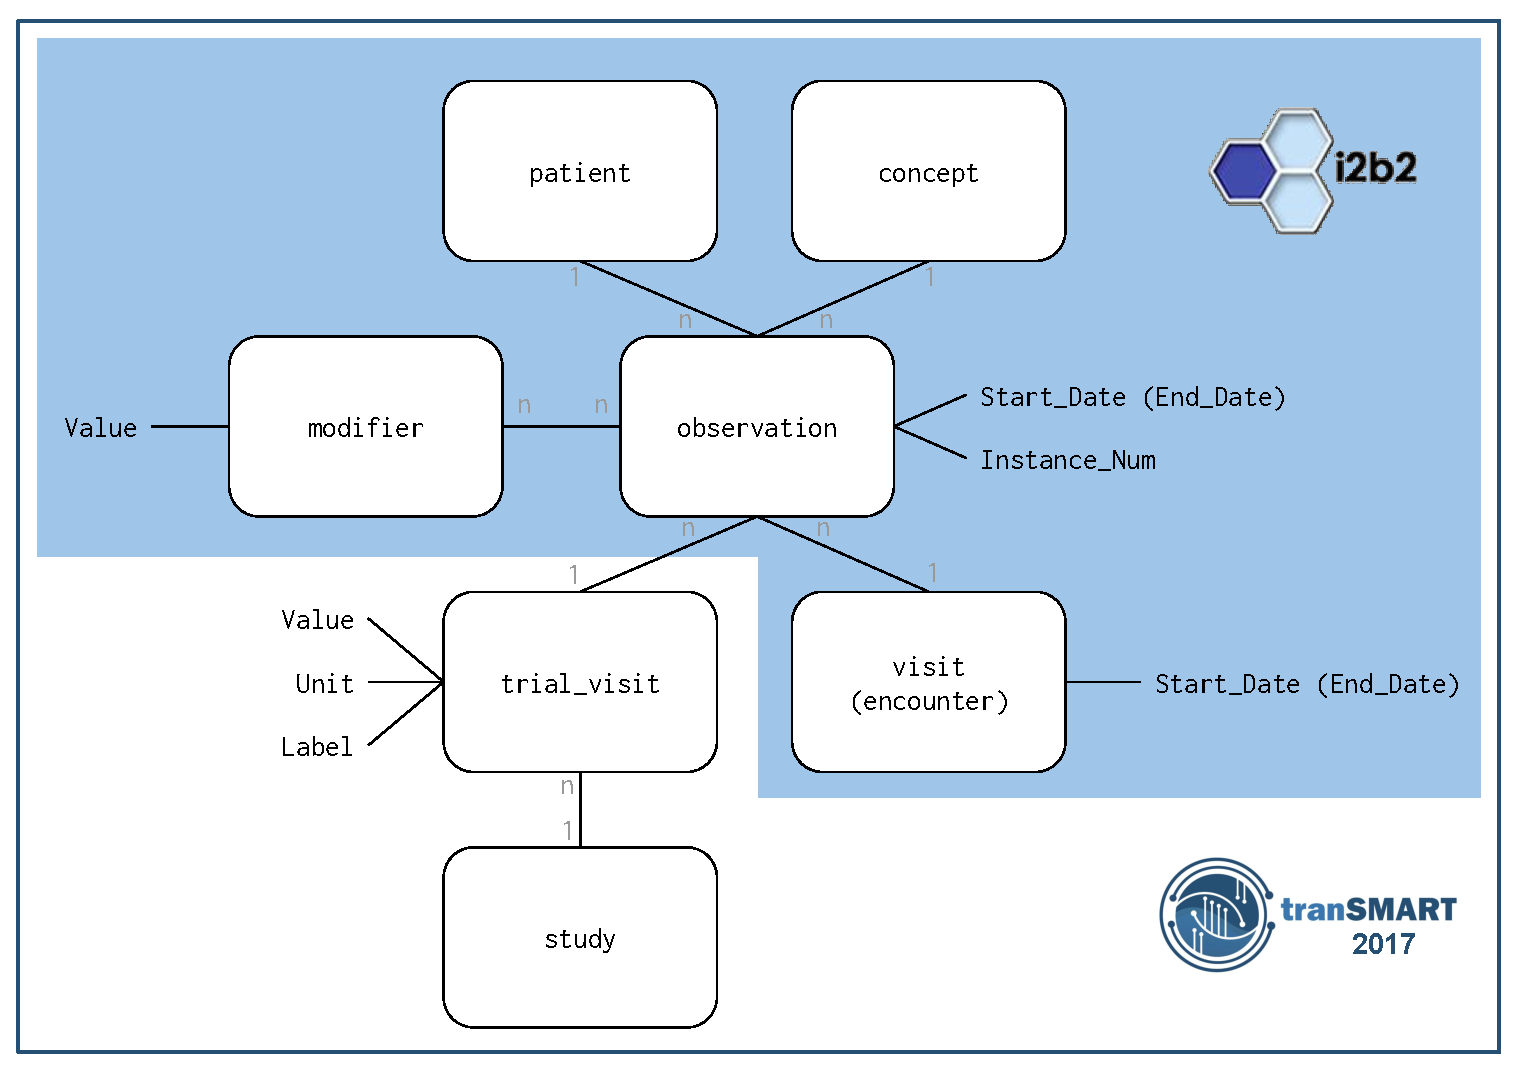
\includegraphics[width=1\textwidth]{figures/star_schema.pdf}
    \caption{\emph{i2b2} and \emph{tranSMART} star schemas. Source: \emph{Ward Weistra, The Hyve}}
    \label{fig:star-schema}
\end{figure}

% medco
MedCo~\cite{medco} is a privacy-preserving clinical research platform, and at the time of the project the only one that offers privacy-preserving guarantees.
It enables the sharing of sensitive medical data within a federated group of clinical sites in a privacy-preserving way by using homomorphic encryption and obfuscation techniques.
MedCo fits our requirements and use-cases as it is open-source, based on i2b2, and supports count queries based on inclusion and exclusion criterion, with end-to-end encryption.


\subsection{Front End System: Cohort Explorers}

% requirements for front end
To build our front end we have several systems on which we could base our solution on.
We require it to be modern, open-source, web-based for portability, and if possible at least partially compatible with the clinical research platforms we support.
If all those requirements can not be met, there is left the option of building the front-end from scratch, but as explained in this section we manage to avoid this significant effort.

% list of candidates
The result of a review of available open-source front-end for cohort exploration who deserve to be investigated follows:
\begin{itemize}
    \item i2b2 webclient~\cite{murphy2010serving}~\cite{github:i2b2-webclient}
    \item i2b2 workbench~\cite{murphy2010serving}~\cite{github:i2b2-workbench}
    \item transmartApp~\cite{scheufele2014transmart}~\cite{github:transmartapp}
    \item Glowing Bear~\cite{gb}~\cite{github:gb}
\end{itemize}

% i2b2 webclient / workbench and transmartapp
Each of the previously retained platforms have their official web front end: the \emph{i2b2 webclient} for i2b2, and \emph{tranSMARTApp} for tranSMART.
Both of them are perfectly compatible with their respective back ends, however they suffer from two major problems:
\begin{enumerate*}
    \item they use old or outdated technologies, making future development and maintenance more difficult;
    \item they are very tightly linked to their back end, making the development of support for the other difficult.
\end{enumerate*}
The \emph{i2b2 webclient} uses \emph{yui}~\cite{yui}, a javascript framework developed by Yahoo, and not supported anymore since 2014. 
\emph{tranSMARTApp} is a web application rendered on the server-side in Java, alongside tranSMART, and not a pure web client.
For those reasons we choose to not retain those solutions.
We can also consider the \emph{i2b2 workbench}, client desktop application for i2b2, but as it is not web-based we discard it as well.

% introduce gb yep
\emph{Glowing Bear} is the front end system we choose to retain.
It is modern, web-based and mature software. 
It is implemented on top of tranSMART (v17.1) but its source is structured generically, facilitating the implementation of support for other platforms.
It thus fits all our requirements for a front end.


\subsection{Identity Provider}

Such a system with different components calls for a common and standardized way of handling authentication and authorization.
The de-facto modern standard for this is the OpenID Connect protocol~\cite{rfc:oidc} (OIDC), which we are using in our solution.
OIDC allows to externalize in a secure way authentication and authorization in a multi-components system.
A stable, mature and open-source implementation of OIDC is the server software Keycloak~\cite{keycloak}, that we choose to use.


\section{Building the System Architecture}

\subsection{Assembling the Building Blocks}

% intro
Now that we have the basic building blocks of our solution, we design a system where they fit together in a coherent way.
The architecture can roughly be categorized in three zones:
\begin{itemize}
    \item Front end
    \item Interoperability layer
    \item Clinical research platforms
\end{itemize}
Our building blocks lie in the front end and clinical research platforms zones. 
We now are designing the interoperability layer that connects those two zones.

% assembling
This interoperability layer can be implemented in the front end, in the back end or in both.
Because the front end Glowing Bear implements the compatibility with tranSMART, one possible approach would be to implement the interoperability layer into Glowing Bear by adding the support for i2b2 and MedCo, using the i2b2 XML API, alongside tranSMART.

% front end
However, we want to avoid a fully front end i2b2 API implementation for the following two reasons: 
\begin{enumerate*}
    \item the i2b2 XML API is old and cluttered, which means difficult to implement and maintain;
    \item by only implementing the support for specific systems, this would not leave much space for extensibility.
\end{enumerate*}

% back end
\begin{samepage}
The second option is implementing the layer fully in the back end, which would mean that:
\begin{itemize}
    \item we need a back end component to take care of the APIs translation
    \item the support of tranSMART in Glowing Bear would be removed and re-implemented in the back end component
\end{itemize}
While the first consequence is not a problem, the second implies pretty heavy additional work, with not much added value.
\end{samepage}


% we choose both
For the reasons enumerated before, we choose in our system a hybrid approach: implementing the interoperability layer in both the front end and the back end.
In the front end the support of tranSMART is kept, and we use a back end component to take care of the translation to the other clinical research platforms, i2b2 and MedCo, all the while having Glowing Bear communicating with this component with a unique API.

% pic-sure
For this task the \emph{PIC-SURE} API~\cite{PIC-SURE-API} is the perfect tool.
It is a generic API that was designed to be translated to any kind of API used for querying medical data, and supports several systems, including i2b2.
Although recent, it has been already successfully used to explore data~\cite{patel2016database}.
The back end component implementing the PIC-SURE API is \emph{IRCT} and is open-source.
Thanks to its extensibility capabilities, we are also using it to implement support for MedCo.
Support for the additional systems that IRCT is compatible with is left for future work.

% ccl
To summarize, our interoperability layer is composed of 
\begin{enumerate}
    \item an interoperability module in  Glowing Bear, which has support for both the tranSMART REST API v2, and PIC-SURE;
    \item IRCT, which has support for i2b2 and MedCo.
\end{enumerate} 

\subsection{Technical Choices Summary}

We summarize our technical choices:

\begin{itemize}
    \setlength\itemsep{0em}
    \item Supported clinical research platforms: \emph{i2b2 1.7}, \emph{tranSMART 17.1}, \emph{MedCo}
    \item Interoperability layer for i2b2 and MedCo: \emph{IRCT} (PIC-SURE API)
    \item Front end with support for tranSMART REST API v2 and PIC-SURE: \emph{Glowing Bear}
\end{itemize}


\begin{samepage}
\subsubsection*{Technical Considerations}

Additionally we take into consideration some software engineering good practices, which allow us to meet or alleviate the technical constraints listed in the requirements.
\begin{enumerate}
    \item A practical query run time: the overhead of using our solution compared to the original clinical research platforms should be negligible.
    \item Extensible: building support for additional systems should be facilitated.
    \item Preserve existing user experience: the existing technologies that are used should not be modified in a way that degrades existing features.
    \item Using standards: use existing standard APIs and technologies to the best extent possible.
    \item Quality: produce quality code to facilitate maintenance and encourage reuse.
\end{enumerate}
\end{samepage}


\subsection{System Overview}
\begin{figure}[ht]
    \centering
    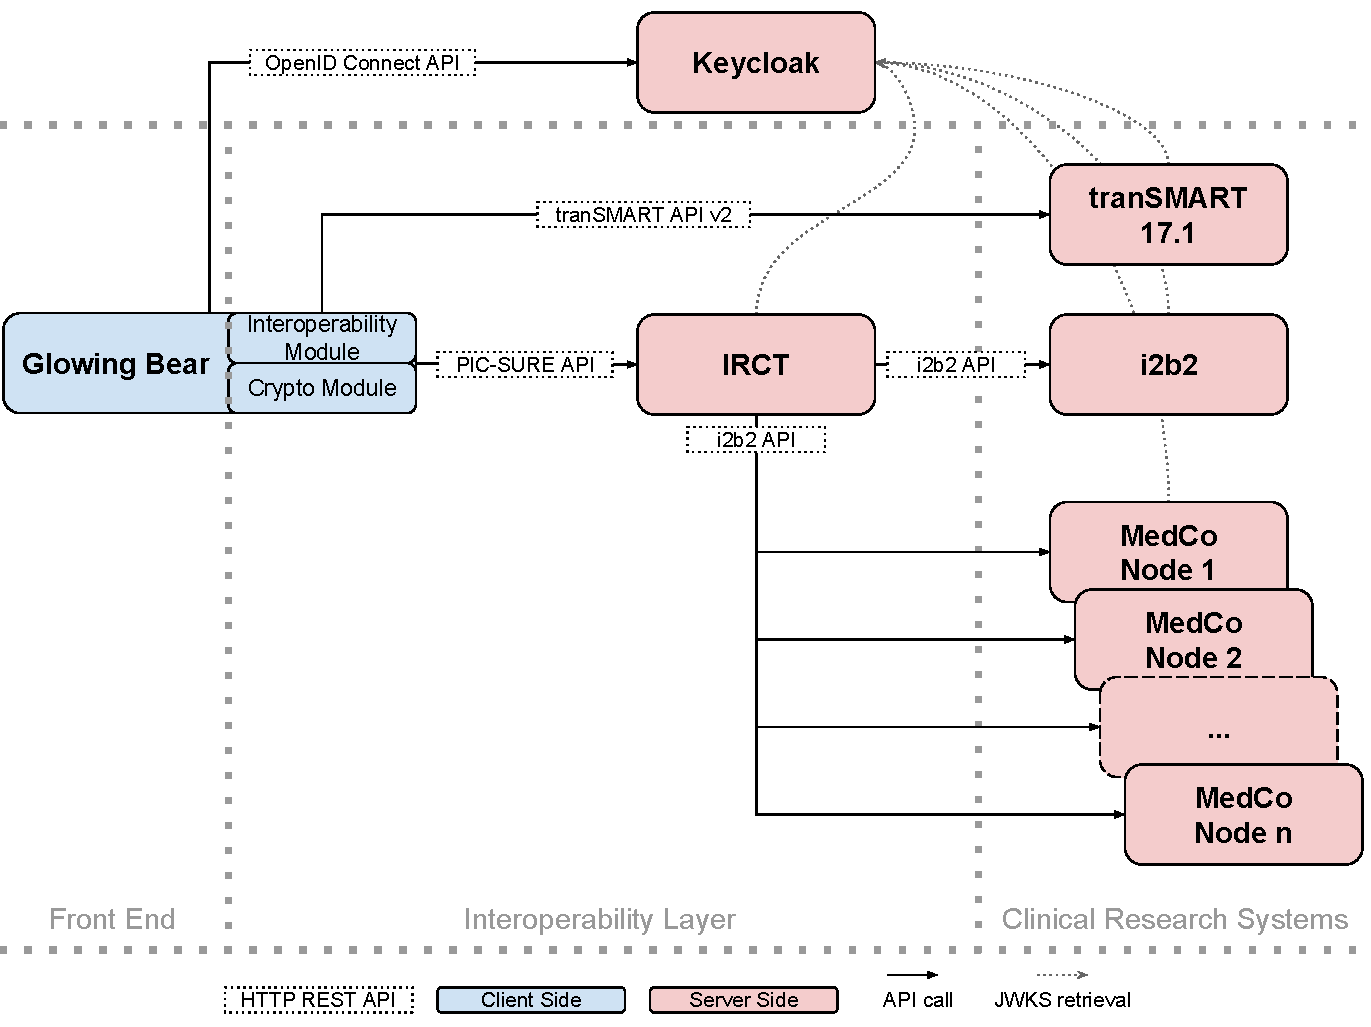
\includegraphics[width=1\textwidth]{figures/sys_diagram_full.pdf}
    \caption{Full System Diagram}
    \label{fig:sys-diagram-full}
\end{figure}

Figure~\ref{fig:sys-diagram-full} shows the architecture of our solution as described in this section.
The high-level idea of the workflow is the following:
\begin{enumerate}
    \item \label{enum:wf-init} While loading Glowing Bear, the user logs in with Keycloak.
    \item The user constructs a query, and Glowing Bear submits it through the appropriate channel:
    \begin{enumerate}
        \item \label{enum:wf-transmart} \emph{tranSMART}: from Glowing Bear, the query is immediately submitted to tranSMART.
        \item \label{enum:wf-i2b2} \emph{i2b2}: from Glowing Bear, the query is submitted to IRCT using the PIC-SURE API, and IRCT submits to i2b2 the query
        \item \label{enum:wf-medco} \emph{MedCo}: using the cryptographic module in Glowing Bear, the query is submitted to IRCT and then broadcasted to all of the MedCo nodes.
    \end{enumerate}
    \item \label{enum:wf-results} The result is fetched and displayed to the user in Glowing Bear. In the case of MedCo the cryptographic module is used to decrypt the result.
\end{enumerate}

The design of step~\ref{enum:wf-init} is covered in section~\ref{sec:interoplayer-idp}, 
step~\ref{enum:wf-i2b2} in section~\ref{sec:interoplayer-gb} and~\ref{sec:interoplayer-picsure}, 
step~\ref{enum:wf-medco} in section~\ref{sec:medco} and finally 
step~\ref{enum:wf-results} in section~\ref{sec:interoplayer-gb}.
Step~\ref{enum:wf-transmart} is not covered in this thesis as the support for tranSMART in Glowing Bear is preexisting.

